\documentclass{article}

% --- Tight PDF output (no standalone.cls needed) ---
\usepackage[
  paperwidth=12cm,
  paperheight=6cm,
  margin=6mm
]{geometry}
\pagestyle{empty}

\usepackage{tikz}
\usetikzlibrary{calc}

\begin{document}
\begin{center}
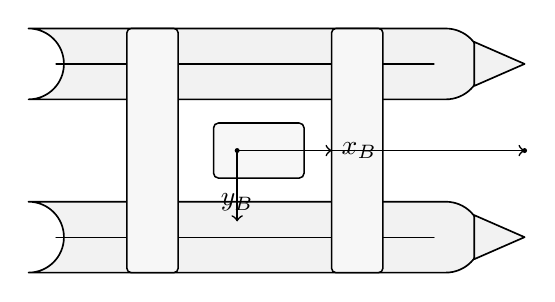
\begin{tikzpicture}[line cap=round, line join=round]

% ---------------- styles ----------------
\tikzset{
  usvHull/.style   ={draw, line width=0.6pt, fill=gray!10},
  usvBeam/.style   ={draw, line width=0.55pt, fill=gray!6},
  usvDetail/.style ={draw, line width=0.45pt},
  usvDot/.style    ={fill=black}
}

% ---------------- parameters (tune once) ----------------
\def\L{6.2}      % pontoon body length (without tip)
\def\W{0.9}      % pontoon width
\def\R{0.45}     % end radius (W/2 recommended)
\def\Tip{0.55}   % bow tip length
\def\Gap{1.1}    % half spacing between pontoons (center-to-center / 2)

% crossbeam geometry
\def\BeamW{0.30} % beam thickness
\def\BeamXf{1.2} % front beam x (relative)
\def\BeamXr{-1.4}% rear beam x (relative)

% derived
\def\xLeft{-\L/2}
\def\xRight{\L/2}
\def\xcL{\xLeft+\R}
\def\xcR{\xRight-\R}
\def\yTop{\W/2}
\def\yBot{-\W/2}

% helper: draw one pontoon centered at (0,y0)
\newcommand{\Pontoon}[1]{%
  % capsule hull (ONE closed path)
  \path[usvHull]
    (\xcL, #1+\yTop) -- (\xcR, #1+\yTop)
    arc[start angle=90, end angle=-90, radius=\R]
    -- (\xcL, #1+\yBot)
    arc[start angle=-90, end angle=90, radius=\R]
    -- cycle;

  % bow tip (triangle)
  \path[usvHull]
    (\xRight-\R*0.20, #1-0.28) -- (\xRight+\Tip, #1) -- (\xRight-\R*0.20, #1+0.28) -- cycle;

  % subtle centerline
  \draw[usvDetail] (\xLeft+0.8, #1) -- (\xRight-0.6, #1);
}

% ---------------- draw two pontoons ----------------
\Pontoon{\Gap}
\Pontoon{-\Gap}

% ---------------- crossbeams (connect pontoons) ----------------
% rear beam
\path[usvBeam, rounded corners=1.5pt]
  (\BeamXr, -\Gap-\W/2) rectangle (\BeamXr+0.65, \Gap+\W/2);
% front beam
\path[usvBeam, rounded corners=1.5pt]
  (\BeamXf, -\Gap-\W/2) rectangle (\BeamXf+0.65, \Gap+\W/2);

% optional: small "payload/deck" block in center
\path[usvBeam, rounded corners=1.8pt]
  (-0.30, -0.35) rectangle (0.85, 0.35);

% ---------------- anchors (for later composition) ----------------
\coordinate (usvCenter) at (0,0);
\coordinate (usvBow)    at (\xRight+\Tip,0);
\coordinate (usvStern)  at (\xLeft,0);

\fill[usvDot] (usvCenter) circle (0.9pt);
\fill[usvDot] (usvBow)    circle (0.9pt);

\draw[->, line width=0.6pt] (usvCenter) -- ++(1.2, 0) node[right] {$x_B$};
\draw[->, line width=0.6pt] (usvCenter) -- ++(0, -0.9) node[above] {$y_B$};

% 艏向角
\draw[->, line width=0.6pt] (usvCenter) -- (usvBow);

\end{tikzpicture}
\end{center}


\end{document}